\documentclass[12pt]{article}

\usepackage{fullpage}
\usepackage[round,numbers]{natbib}
\usepackage{multirow}
\usepackage{booktabs}
\usepackage{graphicx}
\usepackage[toc,page]{appendix}
\usepackage{hyperref}
\usepackage[usenames,dvipsnames]{xcolor}

\hypersetup{
      colorlinks=true,       % false: boxed links; true: colored links
    linkcolor=red,          
   % color of internal links (change box color with linkbordercolor)
    citecolor=green,        % color of links to bibliography
    filecolor=magenta,      % color of file links
    urlcolor=cyan           % color of external links
}


%% Comments
\newif\ifcomments\commentstrue

\ifcomments
\newcommand{\authornote}[3]{\textcolor{#1}{[#3 ---#2]}}
\newcommand{\todo}[1]{\textcolor{red}{[TODO: #1]}}
\else
\newcommand{\authornote}[3]{}
\newcommand{\todo}[1]{}
\fi

\newcommand{\wss}[1]{\authornote{magenta}{SS}{#1}}
\newcommand{\nd}[1]{\authornote{blue}{ND}{#1}}
\newcommand{\ah}[1]{\authornote{violet}{AH}{#1}}

\newcounter{acnum}
\newcommand{\actheacnum}{AC\theacnum}
\newcommand{\acref}[1]{AC\ref{#1}}

\newcounter{ucnum}
\newcommand{\uctheucnum}{UC\theucnum}
\newcommand{\uref}[1]{UC\ref{#1}}

\newcounter{mnum}
\newcommand{\mthemnum}{M\themnum}
\newcommand{\mref}[1]{M\ref{#1}}

\newcommand{\progname}{PolyHarmonics}



\begin{document}

\title{Module Guide for \progname{}} 
\author{Nolan Driessen}
\date{\today}
	
\maketitle

\tableofcontents

\newpage

\section{Introduction}

Decomposing a system into modules is a commonly accepted approach to developing
software.  A module is a work assignment for a programmer or programming
team~\citep{ParnasEtAl1984}.  In the best practices for scientific computing,
\citet{WilsonEtAl2013} advise a modular design, but are silent on the criteria
to use to decompose the software into modules.  We advocate a decomposition
based on the principle of information hiding~\citep{Parnas1972a}.  This
principle supports design for change, because the ``secrets'' that each module
hides represent likely future changes.  Design for change is valuable in SC,
where modifications are frequent, especially during initial development as the
solution space is explored.  

Our design follows the rules laid out by \citet{ParnasEtAl1984}, as follows:
\begin{itemize}
\item System details that are likely to change independently should be the
  secrets of separate modules.
\item Each data structure is used in only one module.
\item Any other program that requires information stored in a module's data
  structures must obtain it by calling access programs belonging to that module.
\end{itemize}

After completing the first stage of the design, the Software Requirements
Specification (SRS), the Module Guide (MG) is developed~\citep{ParnasEtAl1984}. 
The MG
specifies the modular structure of the system and is intended to allow both
designers and maintainers to easily identify the parts of the software.  The
potential readers of this document are as follows:

\begin{itemize}
\item New project members: This document can be a guide for a new project member
  to easily understand the overall structure and quickly find the
  relevant modules they are searching for.
\item Maintainers: The hierarchical structure of the module guide improves the
  maintainers' understanding when they need to make changes to the system. It is
  important for a maintainer to update the relevant sections of the document
  after changes have been made.
\item Designers: Once the module guide has been written, it can be used to
  check for consistency, feasibility and flexibility. Designers can verify the
  system in various ways, such as consistency among modules, feasibility of the
  decomposition, and flexibility of the design.
\end{itemize}

The rest of the document is organized as follows. Section
\ref{SecChange} lists the anticipated and unlikely changes of the software
requirements. Section \ref{SecMH} summarizes the module decomposition that
was constructed according to the likely changes. Section \ref{SecConnection}
specifies the connections between the software requirements and the
modules. Section \ref{SecMD} gives a detailed description of the
modules. Section \ref{SecTM} includes two traceability matrices. One checks
the completeness of the design against the requirements provided in the SRS. The
other shows the relation between anticipated changes and the modules. Section
\ref{SecUse} describes the use relation between modules.

\section{Anticipated and Unlikely Changes} \label{SecChange}

This section lists possible changes to the system. According to the likeliness
of the change, the possible changes are classified into two
categories. Anticipated changes are listed in Section \ref{SecAchange}, and
unlikely changes are listed in Section \ref{SecUchange}.

\subsection{Anticipated Changes} \label{SecAchange}

Anticipated changes are the source of the information that is to be hidden
inside the modules. Ideally, changing one of the anticipated changes will only
require changing the one module that hides the associated decision. The approach
adapted here is called design for
change. %Anticipated changes are numbered by \textbf{AC} followed by a number.

\begin{description}
\item[\refstepcounter{acnum} \actheacnum \label{acHardware}:] The specific
  hardware on which the software is running.
\item[\refstepcounter{acnum} \actheacnum \label{acOutput}:] The information 
contained within the output text files.
\item[\refstepcounter{acnum} \actheacnum \label{acFileFinding}:] The method of 
finding and using input files.
\item[\refstepcounter{acnum} \actheacnum \label{acFileStoring}:] The method of 
storing required information found within input files.
\item[\refstepcounter{acnum} \actheacnum \label{acPlot}:] The way the plots are 
created and displayed.
\item[\refstepcounter{acnum} \actheacnum \label{acAnalyze}:] The components of 
the signal being analyzed.
\item[\refstepcounter{acnum} \actheacnum \label{acMethod}:] The method used for 
analysis of the acoustic signals.
\item[\refstepcounter{acnum} \actheacnum \label{acControl}:] The control flow of 
the system.
\item[\refstepcounter{acnum} \actheacnum \label{acFilter}:] The method of 
filtering the input data.
\item[\refstepcounter{acnum} \actheacnum \label{acFilterInfo}:] The method of 
storing the filtered data.
\end{description}


\subsection{Unlikely Changes} \label{SecUchange}

The module design should be as general as possible. However, a general system is
more complex. Sometimes this complexity is not necessary. Fixing some design
decisions at the system architecture stage can simplify the software design. If
these decision should later need to be changed, then many parts of the design
will potentially need to be modified. Hence, it is not intended that these
decisions will be changed. 

% As an example, the ODEs for the temperature and the
%energy equations are assumed to follow the structure given in the SRS; that is,
%even if they need to be modified, the modifications should be possible by
%changing how the input parameters are used in the definition.  If new 
%parameters
%are needed, this will mean a change to both the input parameters module, the
%calculation module and the output module.

\begin{description}
\item[\refstepcounter{ucnum} \uctheucnum \label{ucIO}:] Input/Output devices
  (Input: Keyboard and/or mouse, Output: Memory and/or Screen).
\item[\refstepcounter{ucnum} \uctheucnum \label{ucOutput}:] Output data is
  displayed to the output device.
\item[\refstepcounter{ucnum} \uctheucnum \label{ucGoal}:] The goal of the system
  is to interpret acoustic signals.
\item[\refstepcounter{ucnum} \uctheucnum \label{ucDFT}:] The Discrete Fourier 
Transform is used.
\item[\refstepcounter{ucnum} \uctheucnum \label{ucInput}:] The system receives 
input from a LabVIEW TDMS file as described by section 4.2 in the Software
 Requirements Specification. 
\item[\refstepcounter{ucnum} \uctheucnum \label{ucPlot}:] Plots are created 
containing critical information regarding the signals analyzed.
\item[\refstepcounter{ucnum} \uctheucnum \label{ucProMV}:] The system gives 
its output to ProMV after analysis as described by section 4.2 in the Software
 Requirements Specification. \wss{You could reference the system constraints
  in the SRS at this point.}
  
  \nd{Both spots referenced}
\end{description}

\section{Module Hierarchy} \label{SecMH}

This section provides an overview of the module design. Modules are summarized
in a hierarchy decomposed by secrets in Table \ref{TblMH}. The modules listed
below, which are leaves in the hierarchy tree, are the modules that will
actually be implemented.

\begin{description}
\item [\refstepcounter{mnum} \mthemnum \label{mHH}:] Hardware-Hiding Module
\item [\refstepcounter{mnum} \mthemnum \label{mInput}:] Input Finding Module
\item [\refstepcounter{mnum} \mthemnum \label{mInputData}:] Input Data Module
\item [\refstepcounter{mnum} \mthemnum \label{mTransformInfo}:] Transformed 
Signal Data Module
\item [\refstepcounter{mnum} \mthemnum \label{mTransform}:] Signal 
Transforming Module
\item [\refstepcounter{mnum} \mthemnum \label{mPlotInfo}:] Plot Data Module
\item [\refstepcounter{mnum} \mthemnum \label{mControl}:] Control Module
\item [\refstepcounter{mnum} \mthemnum \label{mOutput}:] Output Module
\item [\refstepcounter{mnum} \mthemnum \label{mFilter}:] Filtering Module
\item [\refstepcounter{mnum} \mthemnum \label{mFilterInfo}:] Filtered Data
 Module
\end{description}

Note that \mref{mHH} is a commonly used module and is already implemented by the 
operating
system.  It will not be reimplemented.

\begin{table}[h!]
\centering
\caption{Module Hierarchy}
\begin{tabular}{p{0.3\textwidth} p{0.4\textwidth} p{0.3\textwidth}}
\toprule
\textbf{Level 1} & \textbf{Level 2} & \textbf{Level 3}\\
\midrule

{Hardware-Hiding Module} & ~ \\
\midrule
\multirow{7}{0.3\textwidth}{Behaviour-Hiding Module}
& \multirow{2}{0.3\textwidth}{Input Module} 
& Input Finding Module\\
& & Input Data Module\\  
& Transformed Signal Data Module\\ 
& Plot Data Module\\ 
& Control Module\\ 
& Output Module\\ 
& Filtered Data Module\\
\midrule
\multirow{3}{0.3\textwidth}{Software Decision Module}
&Signal Transforming Module\\ 
& Filtering Module\\
\bottomrule
\end{tabular}
\label{TblMH}
\end{table}

\section{Connection Between Requirements and Design} \label{SecConnection}

The design of the system is intended to satisfy the requirements developed in
the SRS. In this stage, the system is decomposed into modules. The connection
between requirements and modules is listed in Table \ref{TblRT}.

\section{Module Decomposition} \label{SecMD}
Modules are decomposed according to the principle of ``information hiding''
proposed by \citet{ParnasEtAl1984}. The \emph{Secrets} field in a module
decomposition is a brief statement of the design decision hidden by the
module. The \emph{Services} field specifies \emph{what} the module will do
without documenting \emph{how} to do it. For each module, a suggestion for the
implementing software is given under the \emph{Implemented By} title. If the
entry is \emph{OS}, this means that the module is provided by the operating
system or by standard programming language libraries. If the entry is
\progname{}, this means that the module will be implemented by the 
acoustic analysis software. If the entry is \emph{NumPy}, \emph{Matplotlib} or
 \emph{Pywt} it means the module will be implemented by that specific Python 
library. If a dash (\emph{--}) is shown, this means
that the module is not a leaf and will not have to be implemented. Whether or
not this module is implemented depends on the programming language
selected.

\subsection{Hardware Hiding Modules (\mref{mHH})}

\begin{description}
\item[Secrets:]The data structure and algorithm used to implement the virtual
  hardware.
\item[Services:]Serves as a virtual hardware used by the rest of the
  system. This module provides the interface between the hardware and the
  software. So, the system can use it to display outputs or to accept inputs.
\item[Implemented By:] OS
\end{description}

\subsection{Behaviour-Hiding Module}

\begin{description}
\item[Secrets:]The contents of the required behaviors.
\item[Services:]Includes programs that provide externally visible behavior of
  the system as specified in the software requirements specification (SRS)
  documents. This module serves as a communication layer between the
  hardware-hiding module and the software decision module. The programs in this
  module will need to change if there are changes in the SRS.
\item[Implemented By:] --
\end{description}

\subsubsection{Input Finding Module  (\mref{mInput})}	
\begin{description}
\item[Secrets:]Encapsulates finding files for input and accepting user input.
\item[Services:]Searches for TDMS files within the given directory and accepts 
starting stopping and step frequencies from the user.
\item[Implemented By:] \progname{}
\end{description}

\subsubsection{Input Data Module  (\mref{mInputData})}
\begin{description}
\item[Secrets:]The format and structure of the data found within the input 
files.
\item[Services:]Stores the data from the Input Module.
\item[Implemented By:] \progname{}
\end{description}
		
\subsubsection{Transformed Signal Data Module (\mref{mTransformInfo})}
\begin{description}
\item[Secrets:] The format and structure of the data of the transformed signal.
\item[Services:] Stores the data of the transformed signal.
\item[Implemented By:] \progname{}
\end{description}

\subsubsection{Plot Data Module (\mref{mPlotInfo})}
\begin{description}
\item[Secrets:] Encapsulates the creation of plots.
\item[Services:] Creates plots of the input data and transformed data.
\item[Implemented By:] \progname{}
\end{description}

\subsubsection{Control Module (\mref{mControl})}
\begin{description}
\item[Secrets:] The algorithm for coordinating the running of the program.
\item[Services:] Provides the main program.
\item[Implemented By:] \progname{}
\end{description}

\subsubsection{Output Module (\mref{mOutput})}
\begin{description}
\item[Secrets:] The format and structure of the output data.
\item[Services:] Writes the output data to the output files in the proper 
format.
\item[Implemented By:] \progname{}
\end{description}

\subsubsection{Filtered Data (\mref{mFilterInfo})}
\begin{description}
\item[Secrets:] The format and structure of the filtered data.
\item[Services:] Stores the data of the filtered signal.
\item[Implemented By:] \progname{}
\end{description}
\subsection{Software Decision Module}

\begin{description}
\item[Secrets:] The design decisions based on mathematical theorems, physical
  facts, or programming considerations. The secrets of this module are
  \emph{not} described in the SRS.
\item[Services:] Includes data structures and algorithms used in the system that
  do not provide direct interaction with the user. 
  % Changes in these modules are more likely to be motivated by a desire to
  % improve performance than by externally imposed changes.
\item[Implemented By:] --
\end{description}

\subsubsection{Signal Transforming Module (\mref{mTransform})}

\begin{description}
\item[Secrets:] Encapsulates taking an acoustic signal in the time domain and 
transforming it to the frequency domain.
\item[Services:] Handles the algorithm for taking the Discrete Fourier 
Transform.
\item[Implemented By:] NumPy
\end{description}

\subsubsection{Filtering Module (\mref{mFilter})}
\begin{description}
\item[Secrets:] Encapsulates applying a filter to the input data.
\item[Services:] Handles applying the Haar wavelet algorithm.
\item[Implemented By:] Pywt
\end{description}
\section{Traceability Matrix} \label{SecTM}

This section provides two traceability matrices: between the \hyperref[SecMH]{modules} and the
requirements, Table \ref{TblRT}, and between the modules and the
 \hyperref[SecAchange]{anticipated changes}, Table \ref{TblAC}.

% the table should use mref, the requirements should be named, use something
% like fref
\begin{table}[h!]
\centering
\caption{Trace Between Requirements and Modules}
\begin{tabular}{p{0.2\textwidth} p{0.6\textwidth}}
\toprule
\textbf{Req.} & \textbf{Modules}\\
\midrule
R1 & \mref{mHH}, \mref{mInput}, \mref{mControl}\\
R2 & \mref{mInputData}, \mref{mControl}\\
R3 & \mref{mInputData}, \mref{mControl}, \mref{mFilter}, \mref{mFilterInfo}\\
R4 & 
\mref{mInputData}, \mref{mTransformInfo}, \mref{mTransform}, \mref{mControl},
\mref{mFilterInfo}\\
R5 & \mref{mPlotInfo}, \mref{mControl}\\
R6 & \mref{mPlotInfo}, \mref{mControl}\\
R7 & \mref{mPlotInfo}, \mref{mControl}\\
 R8 & \mref{mInputData}, \mref{mControl}, \mref{mOutput}\\
 R9 & \mref{mControl}, \mref{mOutput}, \mref{mFilterInfo}\\
 R10 & \mref{mInputData}, \mref{mControl}, \mref{mOutput}\\
\bottomrule
\end{tabular}
\label{TblRT}
\end{table}

\begin{table}[h!]
\centering
\caption{Trace Between Anticipated Changes and Modules}
\begin{tabular}{p{0.2\textwidth} p{0.6\textwidth}}
\toprule
\textbf{A.C.} & \textbf{Modules}\\
\midrule
AC1 & \mref{mHH}\\
AC2 & \mref{mOutput}\\
AC3 & \mref{mInput}\\
AC4 & \mref{mInputData}\\ 
AC5 & \mref{mPlotInfo}\\
AC6 & \mref{mTransformInfo}\\
AC7 & \mref{mTransform}\\
AC8& \mref{mControl}\\
AC9 & \mref{mFilter}\\
AC10 & \mref{mFilterInfo}\\ 
\bottomrule
\end{tabular}
\label{TblAC}
\end{table}

\section{Use Hierarchy Between Modules} \label{SecUse}

In this section, the uses hierarchy between modules is
provided. \citet{Parnas1978} said of two programs A and B that A {\em uses} B if
correct execution of B may be necessary for A to complete the task described in
its specification. That is, A {\em uses} B if there exist situations in which
the correct functioning of A depends upon the availability of a correct
implementation of B.  Figure \ref{Fig_uses} illustrates the use relation between
the modules. It can be seen that the graph is a directed acyclic graph
(DAG). Each level of the hierarchy offers a testable and usable subset of the
system, and modules in the higher level of the hierarchy are essentially simpler
because they use modules from the lower levels.

\begin{figure}[htbp]
\begin{center}
%\rotatebox{-90}
{
 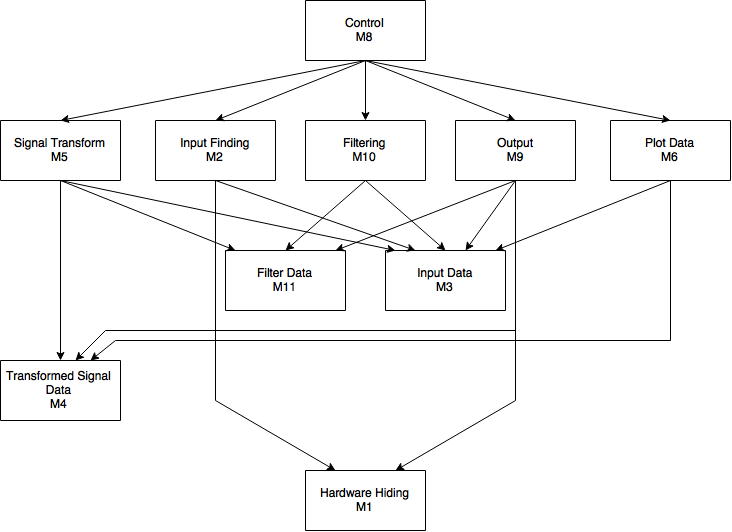
\includegraphics[scale=0.7,trim=1cm 0 0 0]{use.png}
}
\caption{\label{Fig_uses}Use hierarchy among Modules}
\end{center}
\end{figure}

%\section*{References}


\bibliographystyle {plainnat}
\bibliography {../PolyHarmonics_SRS/PolyHarmonics_SRS}
\end{document}




